\section{電源系 (概要/EPS/インヒビット設計(二重絶縁)/電源系統図/電池/SAP)(池谷・中塚)}
\subsection{概要}
本節では本衛星の電源系について述べる.本衛星の電源系の概要を図\ref{3_1_power_diagram}に示す.本衛星の電源系は主に以下のコンポーネントから構成されている.
\begin{itemize}
	\item 太陽電池パネル(Solar Array Panel, SAP)
	\item 電源基板EPS
	\item バッテリ
	\item CIB電源系
	\item 伸展カメラ部電源系
\end{itemize}


% begin{landscape}
% begin{figure}[htbp]
% 	\begin{center}
% 		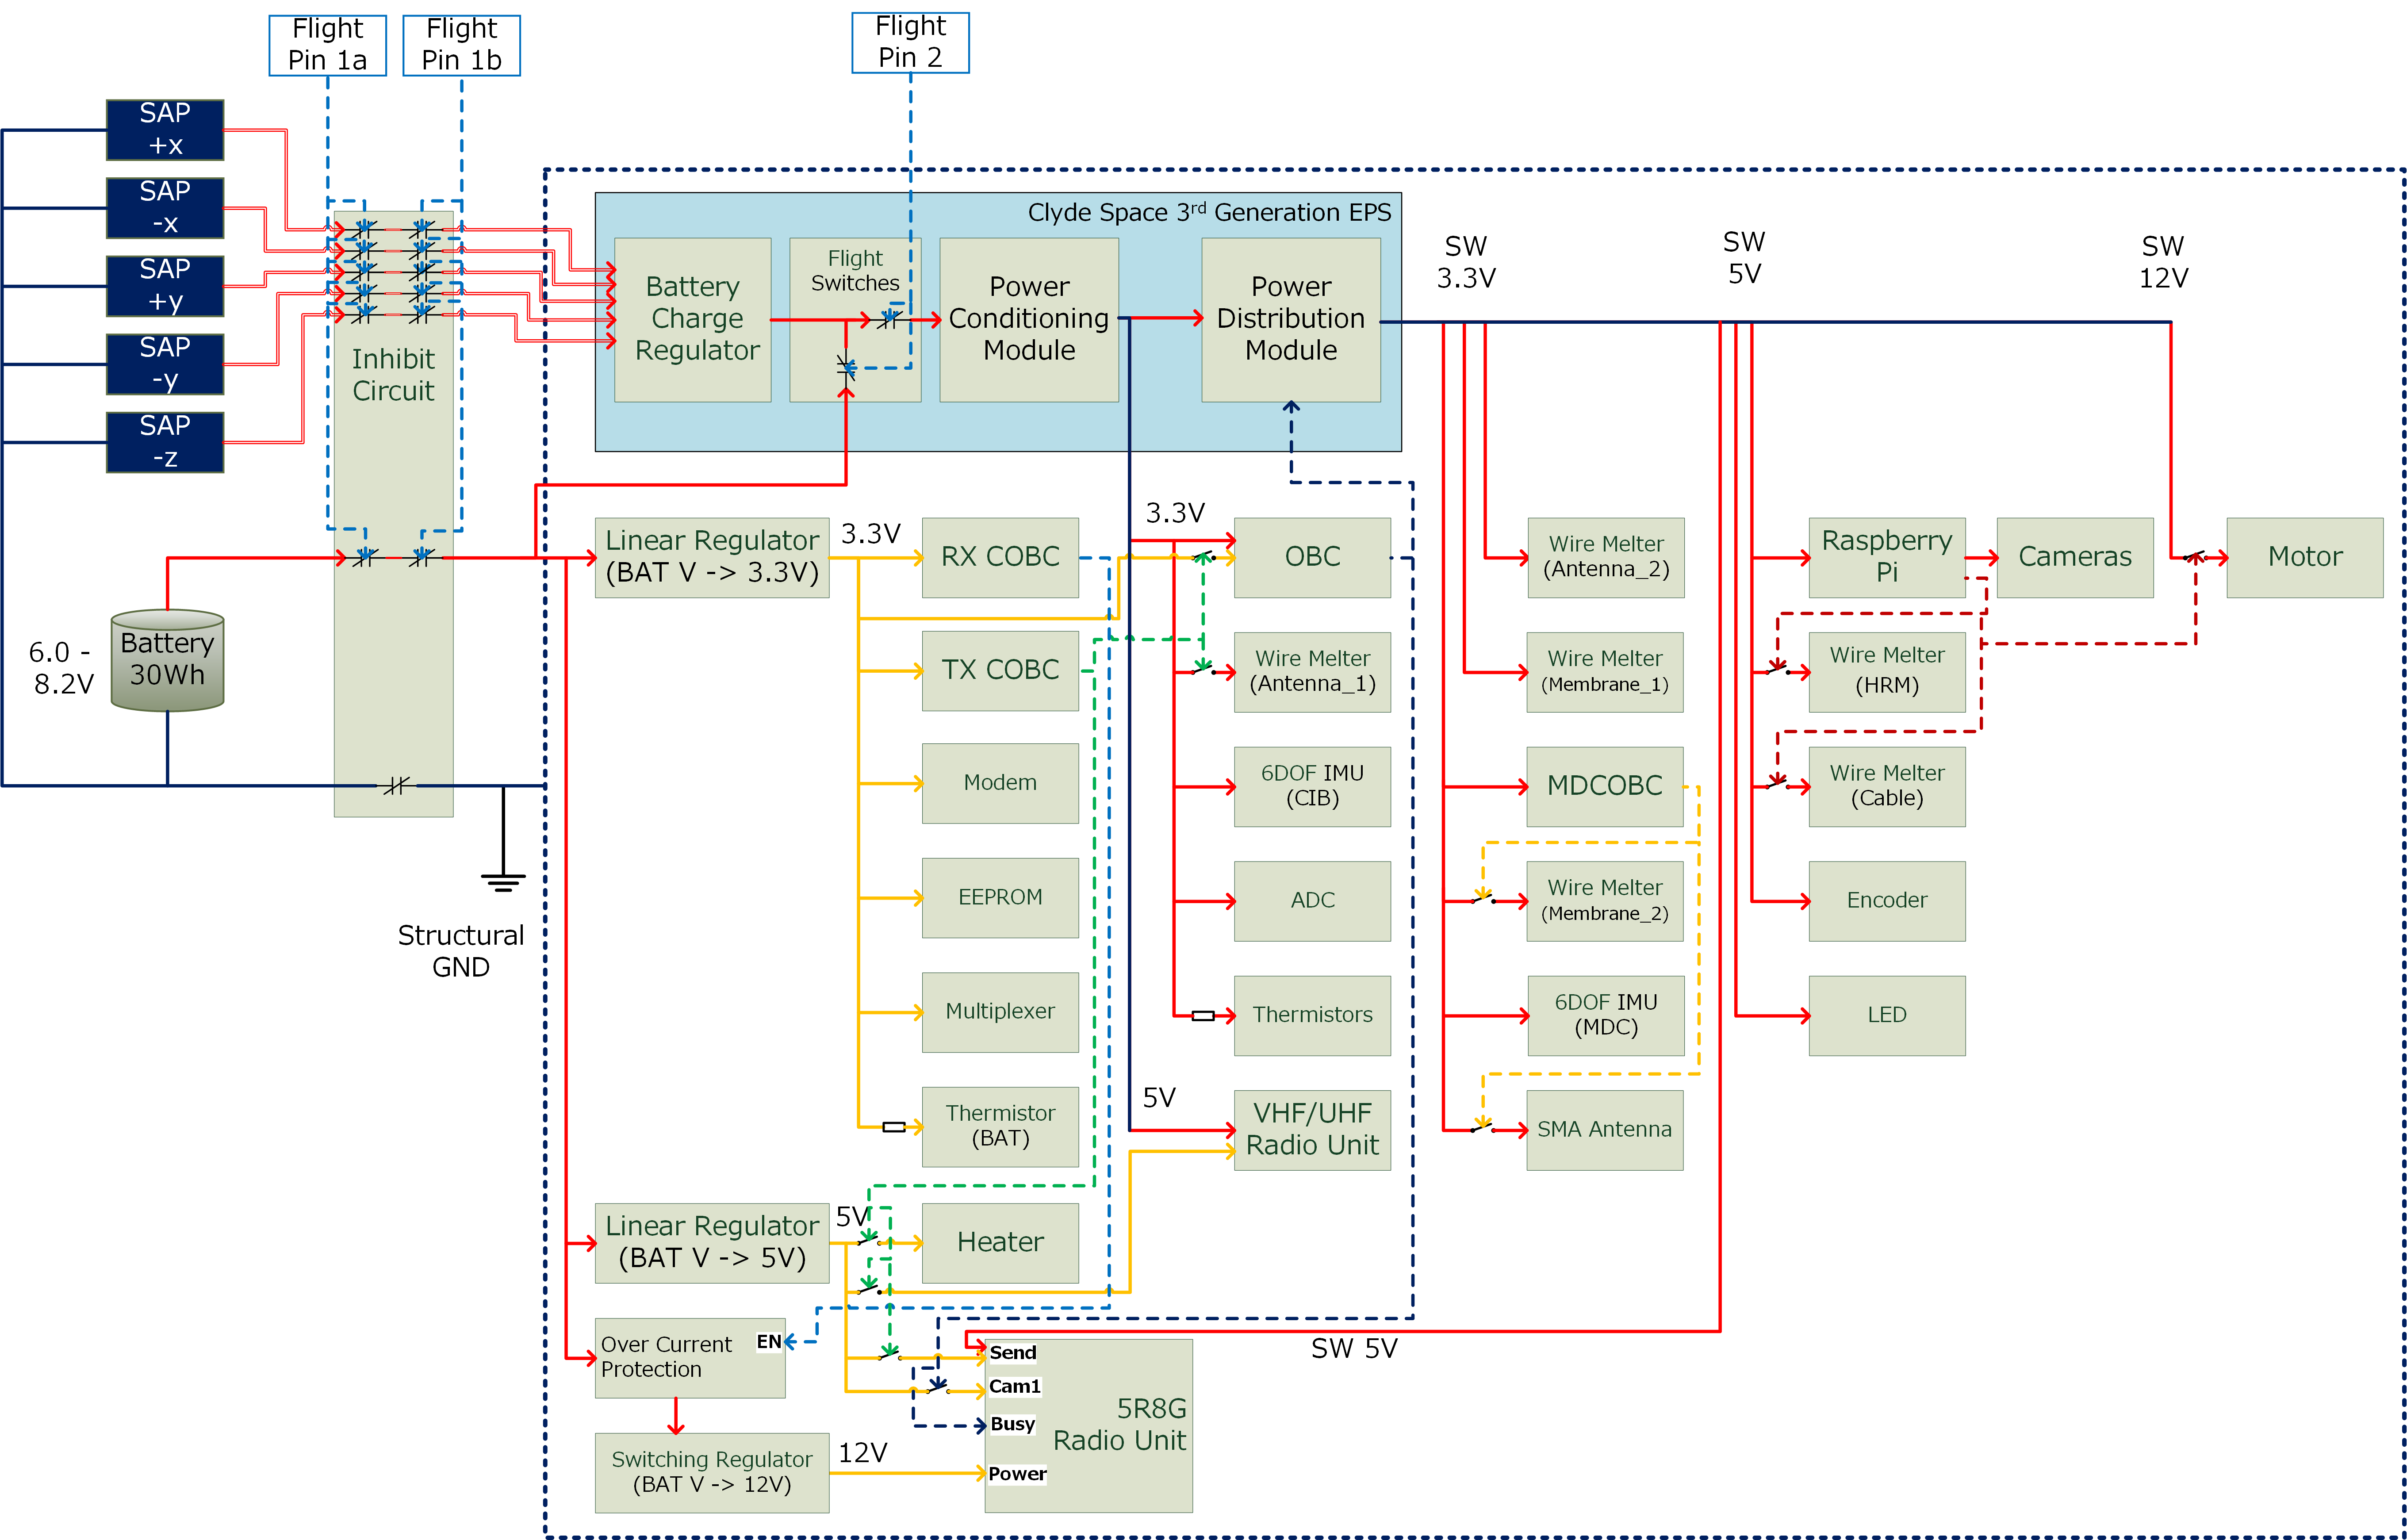
\includegraphics[width=0.5\linewidth]{./03/fig/Power_diagram.png}
%		\caption{Example of a figure caption.}
%		\label{3_1_power_diagram}
%	\end{center}
% \end{figure}
% \end{landscape}            


\subsection{SAP}
\subsubsection{SAP試験}
太陽電池の出力特性試験は,太陽シミュレーターを用いて軌道上と同等の照射強度の光を照射し,太陽電池の電圧-電流特性を測定することで,太陽電池が正常に機能しているかを確認するための試験である.試験により測定した出力特性と,太陽電池セルのデータシート記載の出力特性を比較し確認を行った.出力特性試験は太陽電池セル単体,セルのアレイ化後,アレイの土台への接着後,機体組立後に行った.ただし機体組立後については,正しい測定位置に太陽電池面を持ってくることができなかったため簡易的行った.組立後に正確に測定をするためには別途専用の治具を製作する必要がある.簡易的な試験手順を以下に示す.
\begin{enumerate}
	\item ソーラーシミュレーター(松永研所有)を配電盤に繋いで電源を入れ,15分ほど待機し出力が定常になるのを待つ.
	\item WACOM社のサーモパイル(ソーラーシミュレーター専用放射強度計)とテスターを用いて照射強度の調整を行う.設定方法の詳細はソーラーシミュレーター取扱説明書を参照.本試験では放射強度は1367$\textrm{W}/\textrm{m}^2$である.松永研サーモパイルの変換値は0.017$\textrm{mV}/\textrm{mWcm}^2$である.
	\item 治具の上に測定対象物を乗せた後,扇風機の風を測定対象物に当て温度の定常状態を作る.
	\item 測定対象物の両端子から出ているハーネスをブレッドボードに接続し,間に抵抗を挟んでテスターで出力電圧を測定する.以降抵抗値を変えて測定を繰り返す.
	\item 測定が終了したら取扱説明書に従って太陽シミュレーターの電源を落とす.
\end{enumerate}
また上記の太陽電池出力特性試験とは別に,アレイ化後以降は一部セルを覆って光が当たらないようにした上でアレイの出力を測定し,バイパス機能の確認も行った.

\subsubsection{SAPに関するコメント}
\begin{itemize}
	\item 出力特性試験では,あらかじめ大きなブレッドボード上に試験に使う抵抗を一式用意しておき,ハーネスの接続先を変えるだけの状態で試験をした方がよかった.FM用SAP試験では,残り作業量がわずかだと思っていたため毎回抵抗を付け替えて行っていたが,1回の試験での付け替えには時間がかかる上に,最終的には何かと追加試験をやる機会が増えたため,改善しておけばよかった.
	\item SAP製作及びSAP試験は作業量的には1人いれば十分可能だが,精神衛生上2人以上での作業を勧める.特にSAP出力特性試験では連日3号館101室を真っ暗にして何時間も1人での作業が続き,思っていた以上に負担が大きかった.
	\item SAP製作は非常に時間がかかる上に少しのミスで大きな出戻りが発生する作業である.OrigamiSat-1では太陽電池セルの総枚数が18枚であったためSAP製作が可能であったが,今後の衛星開発でもし太陽電池の枚数を増やすことがあれば,予算との兼ね合いもあるが,SAP製作の外注も検討するべきだと思う.SAPの設計次第ではあるが,太陽電池のセル単位の購入ではなくアレイ化までしてもらった状態での購入も選択肢として存在する.BBMからFMまでで合計何枚の太陽電池セルを発注するか,試験や製作過程で割れた太陽電池セルの枚数,SAPの製作精度等を含めSAP製作のどこを自分達で行うか今後の衛星開発では検討することを勧める.
	\item 太陽シミュレーター及びサーモパイルは非常に高価な機器であるため,取り扱いには特に注意する.また,サーモパイルの管理には注意をすること.一時期サーモパイルが行方不明になっていたようであるが,サーモパイルがなければ正しく放射強度の設定を行うことができず試験にならないため要注意.
\end{itemize}


\subsection{バッテリ}
バッテリはClyde Space社の30Whr Standalone CubeSat Batteryを購入した(図\ref{fig3_1_bat}).バッテリの電気・構造的特性を表\ref{table3_1_bat_spec}に,絶対最大定格を表\ref{table3_1_bat_max}に示す.
公称 7.6V, 放電容量3900mAhr,
2s3p リチウムポリマー電池
UN勧告適合品,NASA標準EP-Wi-
032適合品.

過放電,過充電,内部短絡,外部短
絡保護回路が組み込まれたバッテリ
パック(次ページ).

2つの保護機能については,メーカーから
試験報告書を入手.
上記とは別途,OrigamiSat-1開発チームで
環境試験(振動,衝撃)前後で特性測定の
検査を実施する.

\begin{figure}[htbp]
	\begin{center}
		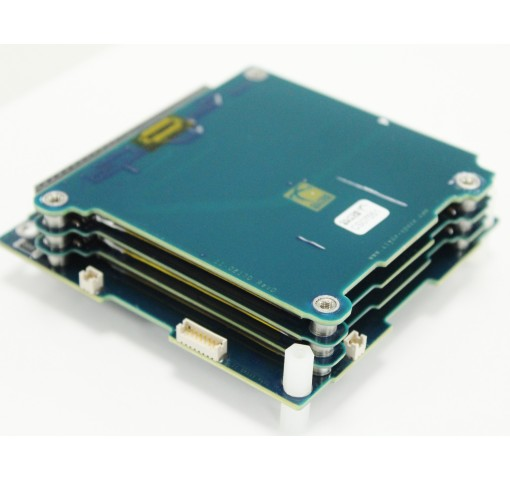
\includegraphics[width=0.5\linewidth]{./03/fig/battery.jpg}
		\caption{30Whr Standalone CubeSat Battery (c)Clyde Space}
		\label{fig3_1_bat}
	\end{center}
\end{figure}

\begin{table}[htbp]
	\begin{center}
		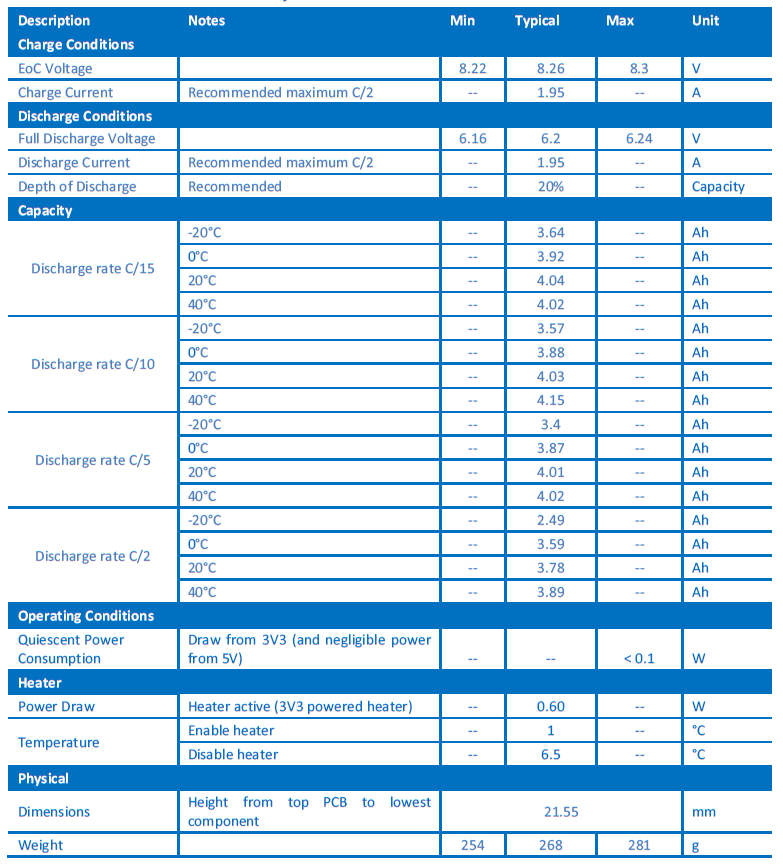
\includegraphics[width=0.8\linewidth]{./03/fig/battery_spec.png}
		\caption{30Whr}
		\label{table3_1_bat_spec}
	\end{center}
\end{table}


\begin{table}
	\caption{Maximum Ratings of the Battery}
	\label{table3_1_bat_max}
	\centering
	\begin{tabular}{ccccc}
		\hline \hline
		\multicolumn{5}{c}{Max Ratings Over Operating Temperature Range (Unless Otherwise Stated)}\\
		&&BCR  & Value  &  Unit  \\
		\hline
		\multirow{3}{*}{Charge Limits}&Voltage&max&8.4&V\\
		&Current&max&6&A\\
		&Current Rate& max &1.53C &Fraction of Capacity\\
		\hline
		\multirow{3}{*}{Discharge Limits}&Voltage&max&6.2&V\\
		&Current&max&6&A\\
		&Current Rate& max &1.53C &Fraction of Capacity\\
		\hline
		\multicolumn{2}{c}{Operating Temperature}&\multicolumn{2}{c}{ -10 to 50} & °C\\
		\multicolumn{2}{c}{\multirow{3}{*}{Storage Temperature}}&\multicolumn{2}{c}{1 Year: -20 to +20}&\multirow{3}{*}{°C}\\
		&&\multicolumn{2}{c}{3 Months: -20 to +45}&\\
		&&\multicolumn{2}{c}{1 Month: -20 to +60}&\\
		\multicolumn{2}{c}{Vacuum}&\multicolumn{2}{c}{10-5}&torr\\
		\multicolumn{2}{c}{Vibration}&\multicolumn{2}{c}{To [RD-3]}\\
		\hline
	\end{tabular}
\end{table}
	

本バッテリは内部保護機能を有しており,


(1) Cell Level Protection Circuit
• 試験結果はCS社提供(「Test Report for Lot
Acceptance Testing」).
• セルごとに配置され,セルは2直列になって
いるので,ユニットとしては2つの保護機能
を有する.

(2) Over-current Polyswitch Protection
(resettable fuse)
• 試験結果(OP-S1-0021 電池セル仕様書、
及び購入先認証状)を入手


\begin{figure}[htbp]
	\begin{center}
		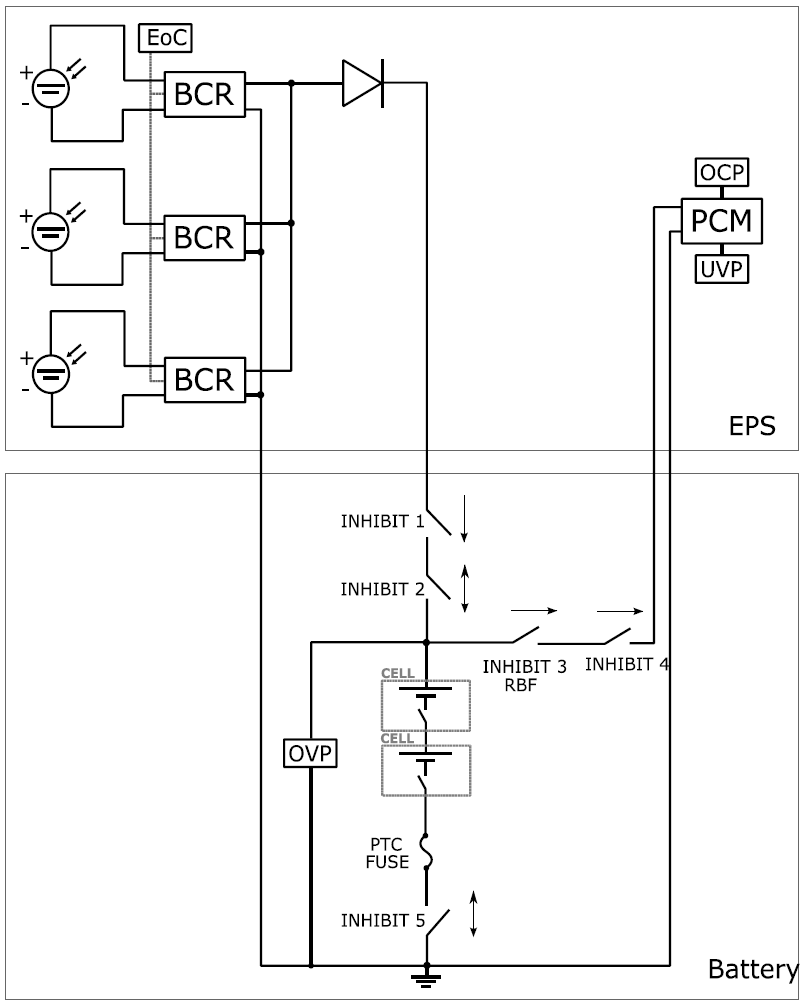
\includegraphics[width=0.5\linewidth]{./03/fig/bat_protection.png}
		\caption{Integrated EPS and Battery Protection Architecture 転載}
		\label{mir}
	\end{center}
\end{figure}

\begin{figure}[htbp]
	\begin{center}
		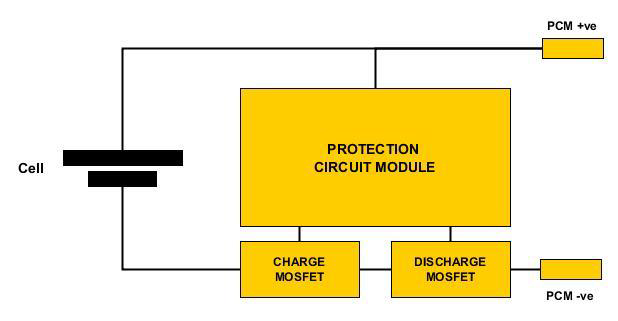
\includegraphics[width=0.5\linewidth]{./03/fig/cell_protection.png}
		\caption{Integrated EPS and Battery Protection Architecture 転載}
		\label{cell_p}
	\end{center}
\end{figure}


\subsection{CIB電源系}

\begin{figure}[htbp]
	\begin{minipage}{0.5\hsize}
		\begin{center}
			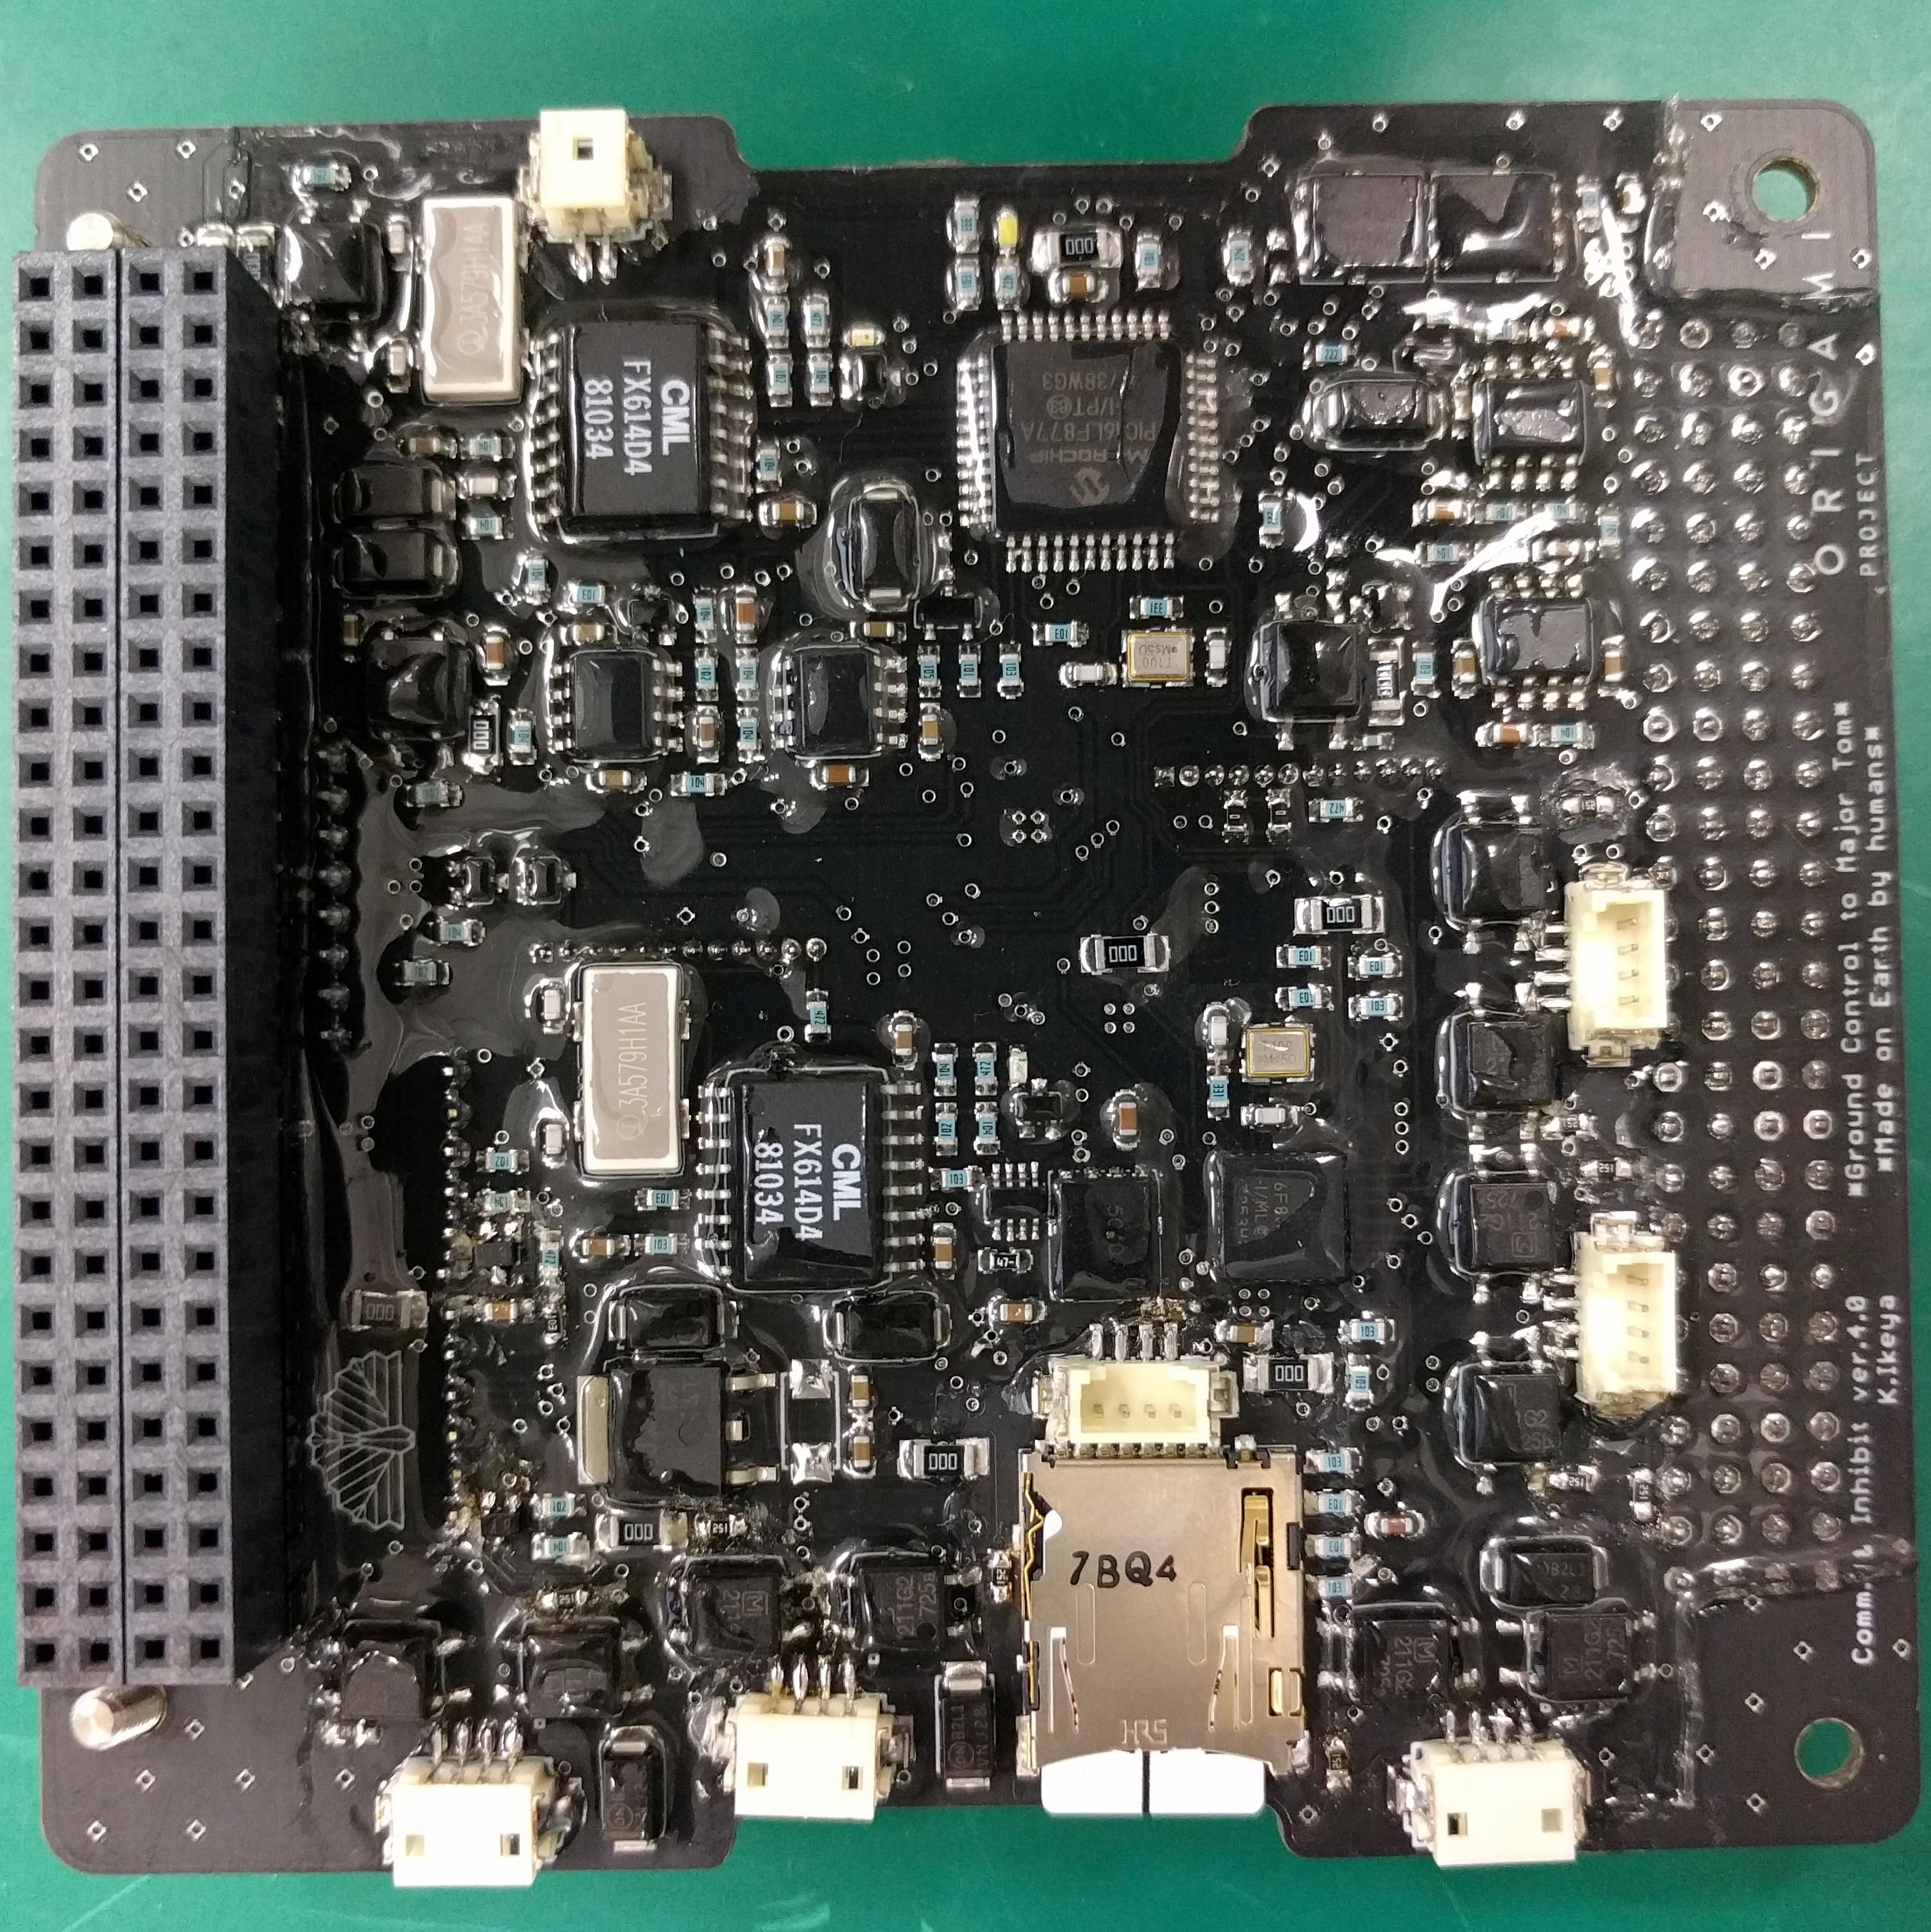
\includegraphics[width=0.7
			\linewidth]{./03/fig/CIB_1.jpg}
		\end{center}
	\end{minipage}
	\begin{minipage}{0.5\hsize}
		\begin{center}
			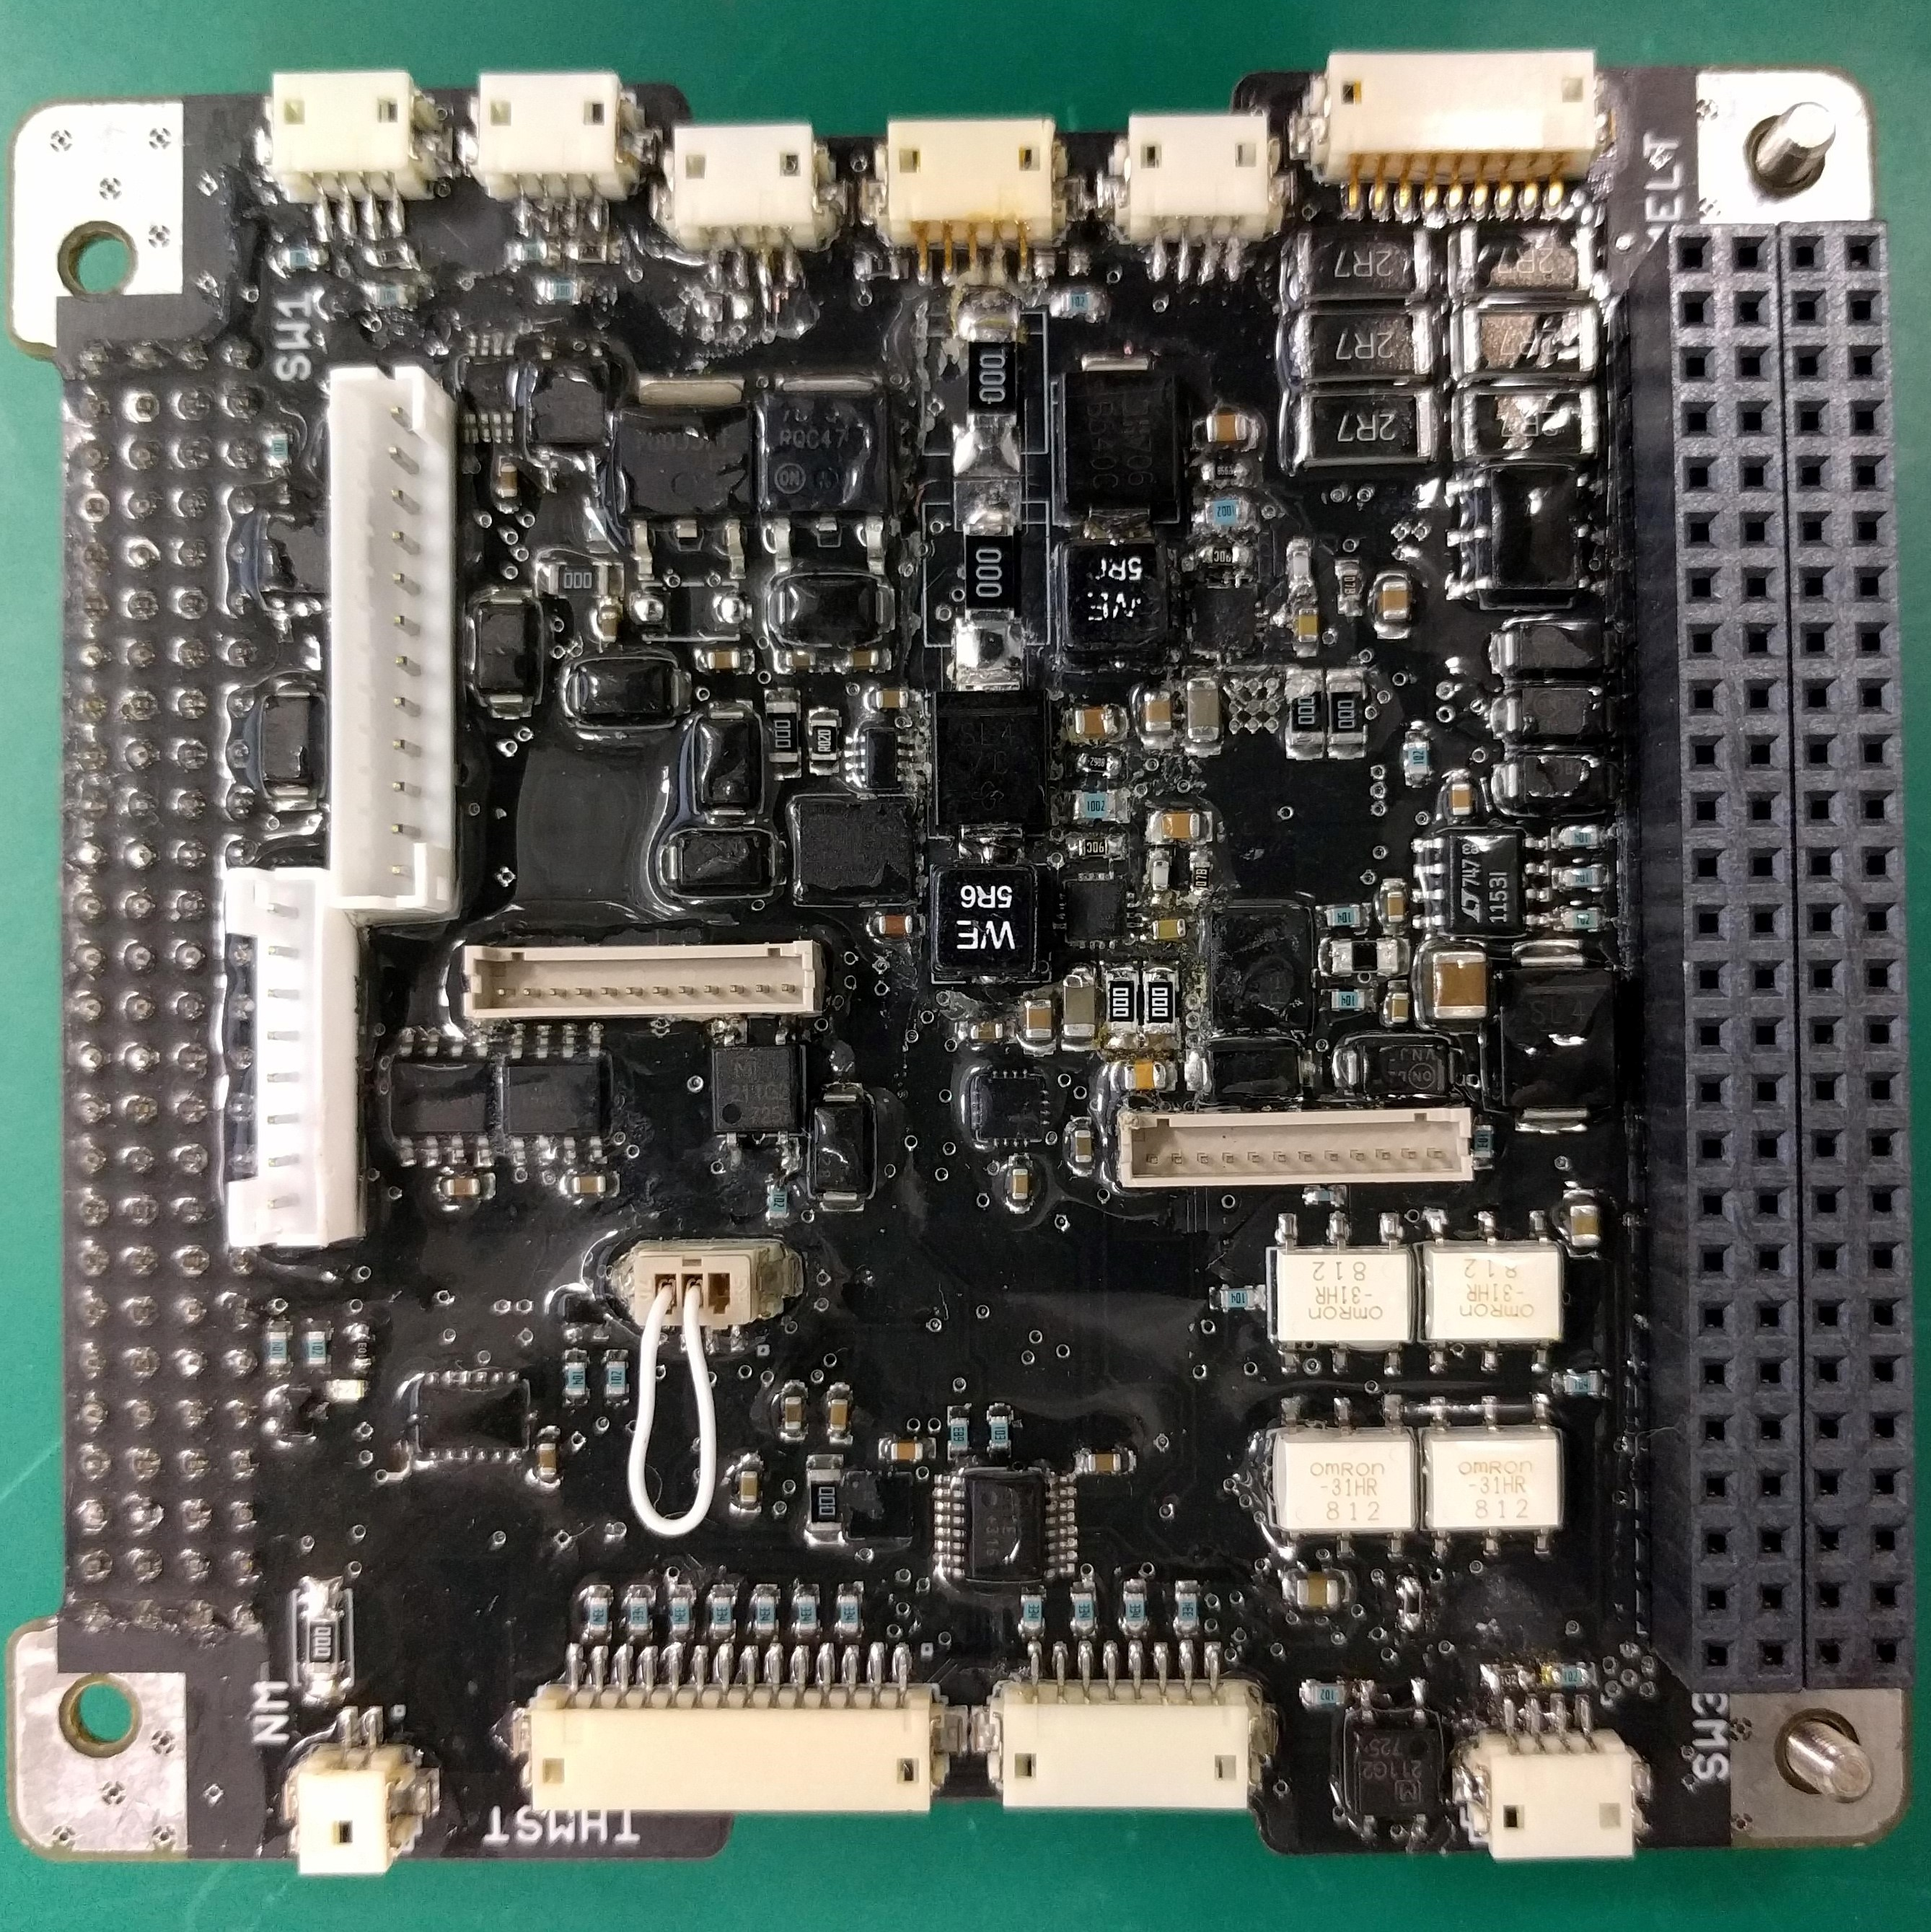
\includegraphics[width=0.7\linewidth]{./03/fig/CIB_2.jpg}
		\end{center}
	\end{minipage}\\		
	\begin{center}
		\caption{CIB}
	\end{center}
\label{CIB}
\end{figure}

\subsubsection{インヒビット回路}
イプシロンロケット


要求により

以下のハザードを設けられた
これらのハザードに対応するために
3インヒビット回路を設けた.

購入品ではこれらの要求を満たせなかったため新たに

Battery-EPS間に新たに

インヒビット回路の回路図は

のようになっている

SAP-EPS間の遮断


\subsubsection{フライトピン}

\subsubsection{CIB内電源回路}
RXCOBCおよびTXCOBCは
UHF/VHF無線機
はほとんどの場合起動していないければならない

そこで新たな電源回路を設けた

三端子レギュレータを並列で繋いだ

そこで二つのレギュレータの出力電流の違いによる
逆流を防止するために
ORダイオード
ダイオードによる電圧降下を防ぐために


また12V系は
突入電流が
購入EPSの

そこで新たにDC-DCコンバータ

これらは二重に

さらに過電流対策

放射線試験によるICの放射線耐性を




\subsection{EPS}
EPSは

を購入した
\begin{figure}[htbp]
	\begin{center}
		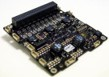
\includegraphics[width=0.5\linewidth]{./03/fig/eps.jpg}
		\caption{EPS}
		\label{eps}
	\end{center}
\end{figure}

\subsection{ミッション部電源系}
ミッション部電源系は
Raspberry Pi
が受け取ったUART信号により
スイッチのON/OFFを切り替える
\ref{}にて
後述する


